\documentclass[twoside]{book}

% Packages required by doxygen
\usepackage{fixltx2e}
\usepackage{calc}
\usepackage{doxygen}
\usepackage[export]{adjustbox} % also loads graphicx
\usepackage{graphicx}
\usepackage[utf8]{inputenc}
\usepackage{makeidx}
\usepackage{multicol}
\usepackage{multirow}
\PassOptionsToPackage{warn}{textcomp}
\usepackage{textcomp}
\usepackage[nointegrals]{wasysym}
\usepackage[table]{xcolor}

% Font selection
\usepackage[T1]{fontenc}
\usepackage[scaled=.90]{helvet}
\usepackage{courier}
\usepackage{amssymb}
\usepackage{sectsty}
\renewcommand{\familydefault}{\sfdefault}
\allsectionsfont{%
  \fontseries{bc}\selectfont%
  \color{darkgray}%
}
\renewcommand{\DoxyLabelFont}{%
  \fontseries{bc}\selectfont%
  \color{darkgray}%
}
\newcommand{\+}{\discretionary{\mbox{\scriptsize$\hookleftarrow$}}{}{}}

% Page & text layout
\usepackage{geometry}
\geometry{%
  a4paper,%
  top=2.5cm,%
  bottom=2.5cm,%
  left=2.5cm,%
  right=2.5cm%
}
\tolerance=750
\hfuzz=15pt
\hbadness=750
\setlength{\emergencystretch}{15pt}
\setlength{\parindent}{0cm}
\setlength{\parskip}{3ex plus 2ex minus 2ex}
\makeatletter
\renewcommand{\paragraph}{%
  \@startsection{paragraph}{4}{0ex}{-1.0ex}{1.0ex}{%
    \normalfont\normalsize\bfseries\SS@parafont%
  }%
}
\renewcommand{\subparagraph}{%
  \@startsection{subparagraph}{5}{0ex}{-1.0ex}{1.0ex}{%
    \normalfont\normalsize\bfseries\SS@subparafont%
  }%
}
\makeatother

% Headers & footers
\usepackage{fancyhdr}
\pagestyle{fancyplain}
\fancyhead[LE]{\fancyplain{}{\bfseries\thepage}}
\fancyhead[CE]{\fancyplain{}{}}
\fancyhead[RE]{\fancyplain{}{\bfseries\leftmark}}
\fancyhead[LO]{\fancyplain{}{\bfseries\rightmark}}
\fancyhead[CO]{\fancyplain{}{}}
\fancyhead[RO]{\fancyplain{}{\bfseries\thepage}}
\fancyfoot[LE]{\fancyplain{}{}}
\fancyfoot[CE]{\fancyplain{}{}}
\fancyfoot[RE]{\fancyplain{}{\bfseries\scriptsize Generated by Doxygen }}
\fancyfoot[LO]{\fancyplain{}{\bfseries\scriptsize Generated by Doxygen }}
\fancyfoot[CO]{\fancyplain{}{}}
\fancyfoot[RO]{\fancyplain{}{}}
\renewcommand{\footrulewidth}{0.4pt}
\renewcommand{\chaptermark}[1]{%
  \markboth{#1}{}%
}
\renewcommand{\sectionmark}[1]{%
  \markright{\thesection\ #1}%
}

% Indices & bibliography
\usepackage{natbib}
\usepackage[titles]{tocloft}
\setcounter{tocdepth}{3}
\setcounter{secnumdepth}{5}
\makeindex

% Hyperlinks (required, but should be loaded last)
\usepackage{ifpdf}
\ifpdf
  \usepackage[pdftex,pagebackref=true]{hyperref}
\else
  \usepackage[ps2pdf,pagebackref=true]{hyperref}
\fi
\hypersetup{%
  colorlinks=true,%
  linkcolor=blue,%
  citecolor=blue,%
  unicode%
}

% Custom commands
\newcommand{\clearemptydoublepage}{%
  \newpage{\pagestyle{empty}\cleardoublepage}%
}

\usepackage{caption}
\captionsetup{labelsep=space,justification=centering,font={bf},singlelinecheck=off,skip=4pt,position=top}

%===== C O N T E N T S =====

\begin{document}

% Titlepage & ToC
\hypersetup{pageanchor=false,
             bookmarksnumbered=true,
             pdfencoding=unicode
            }
\pagenumbering{roman}
\begin{titlepage}
\vspace*{7cm}
\begin{center}%
{\Large My Project }\\
\vspace*{1cm}
{\large Generated by Doxygen 1.8.11}\\
\end{center}
\end{titlepage}
\clearemptydoublepage
\tableofcontents
\clearemptydoublepage
\pagenumbering{arabic}
\hypersetup{pageanchor=true}

%--- Begin generated contents ---
\chapter{Namespace Index}
\section{Packages}
Here are the packages with brief descriptions (if available)\+:\begin{DoxyCompactList}
\item\contentsline{section}{\hyperlink{namespace_plex_byte}{Plex\+Byte} }{\pageref{namespace_plex_byte}}{}
\item\contentsline{section}{\hyperlink{namespace_plex_byte_1_1_mo_cap}{Plex\+Byte.\+Mo\+Cap} }{\pageref{namespace_plex_byte_1_1_mo_cap}}{}
\item\contentsline{section}{\hyperlink{namespace_plex_byte_1_1_mo_cap_1_1_backend}{Plex\+Byte.\+Mo\+Cap.\+Backend} }{\pageref{namespace_plex_byte_1_1_mo_cap_1_1_backend}}{}
\end{DoxyCompactList}

\chapter{Hierarchical Index}
\section{Class Hierarchy}
This inheritance list is sorted roughly, but not completely, alphabetically\+:\begin{DoxyCompactList}
\item I\+Disposable\begin{DoxyCompactList}
\item \contentsline{section}{Plex\+Byte.\+Mo\+Cap.\+Backend.\+Backend\+Service}{\pageref{class_plex_byte_1_1_mo_cap_1_1_backend_1_1_backend_service}}{}
\end{DoxyCompactList}
\end{DoxyCompactList}

\chapter{Class Index}
\section{Class List}
Here are the classes, structs, unions and interfaces with brief descriptions\+:\begin{DoxyCompactList}
\item\contentsline{section}{\hyperlink{class_plex_byte_1_1_mo_cap_1_1_interactions_1_1_account}{Plex\+Byte.\+Mo\+Cap.\+Interactions.\+Account} }{\pageref{class_plex_byte_1_1_mo_cap_1_1_interactions_1_1_account}}{}
\item\contentsline{section}{\hyperlink{class_plex_byte_1_1_mo_cap_1_1_interactions_1_1_expense}{Plex\+Byte.\+Mo\+Cap.\+Interactions.\+Expense} }{\pageref{class_plex_byte_1_1_mo_cap_1_1_interactions_1_1_expense}}{}
\item\contentsline{section}{\hyperlink{interface_plex_byte_1_1_mo_cap_1_1_interactions_1_1_i_account}{Plex\+Byte.\+Mo\+Cap.\+Interactions.\+I\+Account} }{\pageref{interface_plex_byte_1_1_mo_cap_1_1_interactions_1_1_i_account}}{}
\item\contentsline{section}{\hyperlink{interface_plex_byte_1_1_mo_cap_1_1_interactions_1_1_i_expense}{Plex\+Byte.\+Mo\+Cap.\+Interactions.\+I\+Expense} }{\pageref{interface_plex_byte_1_1_mo_cap_1_1_interactions_1_1_i_expense}}{}
\item\contentsline{section}{\hyperlink{interface_plex_byte_1_1_mo_cap_1_1_interactions_1_1_i_interaction}{Plex\+Byte.\+Mo\+Cap.\+Interactions.\+I\+Interaction} }{\pageref{interface_plex_byte_1_1_mo_cap_1_1_interactions_1_1_i_interaction}}{}
\item\contentsline{section}{\hyperlink{interface_plex_byte_1_1_mo_cap_1_1_interactions_1_1_i_interaction_factory}{Plex\+Byte.\+Mo\+Cap.\+Interactions.\+I\+Interaction\+Factory} }{\pageref{interface_plex_byte_1_1_mo_cap_1_1_interactions_1_1_i_interaction_factory}}{}
\item\contentsline{section}{\hyperlink{class_plex_byte_1_1_mo_cap_1_1_interactions_1_1_interaction}{Plex\+Byte.\+Mo\+Cap.\+Interactions.\+Interaction} }{\pageref{class_plex_byte_1_1_mo_cap_1_1_interactions_1_1_interaction}}{}
\item\contentsline{section}{\hyperlink{class_plex_byte_1_1_mo_cap_1_1_interactions_1_1_interaction_event_args}{Plex\+Byte.\+Mo\+Cap.\+Interactions.\+Interaction\+Event\+Args} }{\pageref{class_plex_byte_1_1_mo_cap_1_1_interactions_1_1_interaction_event_args}}{}
\item\contentsline{section}{\hyperlink{class_plex_byte_1_1_mo_cap_1_1_interactions_1_1_interaction_factory}{Plex\+Byte.\+Mo\+Cap.\+Interactions.\+Interaction\+Factory} }{\pageref{class_plex_byte_1_1_mo_cap_1_1_interactions_1_1_interaction_factory}}{}
\item\contentsline{section}{\hyperlink{interface_plex_byte_1_1_mo_cap_1_1_interactions_1_1_i_object_factory}{Plex\+Byte.\+Mo\+Cap.\+Interactions.\+I\+Object\+Factory} }{\pageref{interface_plex_byte_1_1_mo_cap_1_1_interactions_1_1_i_object_factory}}{}
\item\contentsline{section}{\hyperlink{interface_plex_byte_1_1_mo_cap_1_1_interactions_1_1_i_project}{Plex\+Byte.\+Mo\+Cap.\+Interactions.\+I\+Project} }{\pageref{interface_plex_byte_1_1_mo_cap_1_1_interactions_1_1_i_project}}{}
\item\contentsline{section}{\hyperlink{interface_plex_byte_1_1_mo_cap_1_1_interactions_1_1_i_survey}{Plex\+Byte.\+Mo\+Cap.\+Interactions.\+I\+Survey} }{\pageref{interface_plex_byte_1_1_mo_cap_1_1_interactions_1_1_i_survey}}{}
\item\contentsline{section}{\hyperlink{interface_plex_byte_1_1_mo_cap_1_1_interactions_1_1_i_survey_option}{Plex\+Byte.\+Mo\+Cap.\+Interactions.\+I\+Survey\+Option} \\*The survey option interface }{\pageref{interface_plex_byte_1_1_mo_cap_1_1_interactions_1_1_i_survey_option}}{}
\item\contentsline{section}{\hyperlink{interface_plex_byte_1_1_mo_cap_1_1_interactions_1_1_i_task}{Plex\+Byte.\+Mo\+Cap.\+Interactions.\+I\+Task} }{\pageref{interface_plex_byte_1_1_mo_cap_1_1_interactions_1_1_i_task}}{}
\item\contentsline{section}{\hyperlink{interface_plex_byte_1_1_mo_cap_1_1_interactions_1_1_i_timeslice}{Plex\+Byte.\+Mo\+Cap.\+Interactions.\+I\+Timeslice} }{\pageref{interface_plex_byte_1_1_mo_cap_1_1_interactions_1_1_i_timeslice}}{}
\item\contentsline{section}{\hyperlink{interface_plex_byte_1_1_mo_cap_1_1_interactions_1_1_i_vote}{Plex\+Byte.\+Mo\+Cap.\+Interactions.\+I\+Vote} \\*The vote interface }{\pageref{interface_plex_byte_1_1_mo_cap_1_1_interactions_1_1_i_vote}}{}
\item\contentsline{section}{\hyperlink{class_plex_byte_1_1_mo_cap_1_1_interactions_1_1_object_factory}{Plex\+Byte.\+Mo\+Cap.\+Interactions.\+Object\+Factory} }{\pageref{class_plex_byte_1_1_mo_cap_1_1_interactions_1_1_object_factory}}{}
\item\contentsline{section}{\hyperlink{class_plex_byte_1_1_mo_cap_1_1_interactions_1_1_project}{Plex\+Byte.\+Mo\+Cap.\+Interactions.\+Project} }{\pageref{class_plex_byte_1_1_mo_cap_1_1_interactions_1_1_project}}{}
\item\contentsline{section}{\hyperlink{class_plex_byte_1_1_mo_cap_1_1_interactions_1_1_survey}{Plex\+Byte.\+Mo\+Cap.\+Interactions.\+Survey} }{\pageref{class_plex_byte_1_1_mo_cap_1_1_interactions_1_1_survey}}{}
\item\contentsline{section}{\hyperlink{class_plex_byte_1_1_mo_cap_1_1_interactions_1_1_survey_option}{Plex\+Byte.\+Mo\+Cap.\+Interactions.\+Survey\+Option} \\*The survey option class, which hold the option text }{\pageref{class_plex_byte_1_1_mo_cap_1_1_interactions_1_1_survey_option}}{}
\item\contentsline{section}{\hyperlink{class_plex_byte_1_1_mo_cap_1_1_interactions_1_1_task}{Plex\+Byte.\+Mo\+Cap.\+Interactions.\+Task} }{\pageref{class_plex_byte_1_1_mo_cap_1_1_interactions_1_1_task}}{}
\item\contentsline{section}{\hyperlink{class_plex_byte_1_1_mo_cap_1_1_interactions_1_1_timeslice}{Plex\+Byte.\+Mo\+Cap.\+Interactions.\+Timeslice} }{\pageref{class_plex_byte_1_1_mo_cap_1_1_interactions_1_1_timeslice}}{}
\item\contentsline{section}{\hyperlink{class_plex_byte_1_1_mo_cap_1_1_interactions_1_1_vote}{Plex\+Byte.\+Mo\+Cap.\+Interactions.\+Vote} \\*This class holds information about a users choice, containing the user and his choice selected }{\pageref{class_plex_byte_1_1_mo_cap_1_1_interactions_1_1_vote}}{}
\end{DoxyCompactList}

\chapter{File Index}
\section{File List}
Here is a list of all files with brief descriptions\+:\begin{DoxyCompactList}
\item\contentsline{section}{D\+:/\+Users/\+Christian\+B/\+Documents/\+\_\+\+H\+F Infomatik/\+Git\+Hub\+\_\+\+Repos/\+Mo\+Cap/\+Plex\+Byte.\+Mo\+Cap/\+Plex\+Byte.\+Mo\+Cap.\+Backend/\hyperlink{_backend_service_8cs}{Backend\+Service.\+cs} }{\pageref{_backend_service_8cs}}{}
\end{DoxyCompactList}

\chapter{Namespace Documentation}
\hypertarget{namespace_plex_byte}{}\section{Plex\+Byte Namespace Reference}
\label{namespace_plex_byte}\index{Plex\+Byte@{Plex\+Byte}}
\subsection*{Namespaces}
\begin{DoxyCompactItemize}
\item 
namespace \hyperlink{namespace_plex_byte_1_1_mo_cap}{Mo\+Cap}
\end{DoxyCompactItemize}

\hypertarget{namespace_plex_byte_1_1_mo_cap}{}\section{Plex\+Byte.\+Mo\+Cap Namespace Reference}
\label{namespace_plex_byte_1_1_mo_cap}\index{Plex\+Byte.\+Mo\+Cap@{Plex\+Byte.\+Mo\+Cap}}
\subsection*{Namespaces}
\begin{DoxyCompactItemize}
\item 
namespace \hyperlink{namespace_plex_byte_1_1_mo_cap_1_1_win_forms}{Win\+Forms}
\end{DoxyCompactItemize}

\hypertarget{namespace_plex_byte_1_1_mo_cap_1_1_backend}{}\section{Plex\+Byte.\+Mo\+Cap.\+Backend Namespace Reference}
\label{namespace_plex_byte_1_1_mo_cap_1_1_backend}\index{Plex\+Byte.\+Mo\+Cap.\+Backend@{Plex\+Byte.\+Mo\+Cap.\+Backend}}
\subsection*{Classes}
\begin{DoxyCompactItemize}
\item 
class \hyperlink{class_plex_byte_1_1_mo_cap_1_1_backend_1_1_backend_service}{Backend\+Service}
\end{DoxyCompactItemize}
\subsection*{Enumerations}
\begin{DoxyCompactItemize}
\item 
enum \hyperlink{namespace_plex_byte_1_1_mo_cap_1_1_backend_acbe18958b9ae9c08f5c2d2c580fbbf2a}{Object\+Type} \{ \hyperlink{namespace_plex_byte_1_1_mo_cap_1_1_backend_acbe18958b9ae9c08f5c2d2c580fbbf2aa8f9bfe9d1345237cb3b2b205864da075}{Object\+Type.\+User}, 
\hyperlink{namespace_plex_byte_1_1_mo_cap_1_1_backend_acbe18958b9ae9c08f5c2d2c580fbbf2aa9e727fdd3aec8274f46685441900280d}{Object\+Type.\+Project}
 \}
\end{DoxyCompactItemize}


\subsection{Enumeration Type Documentation}
\index{Plex\+Byte\+::\+Mo\+Cap\+::\+Backend@{Plex\+Byte\+::\+Mo\+Cap\+::\+Backend}!Object\+Type@{Object\+Type}}
\index{Object\+Type@{Object\+Type}!Plex\+Byte\+::\+Mo\+Cap\+::\+Backend@{Plex\+Byte\+::\+Mo\+Cap\+::\+Backend}}
\subsubsection[{\texorpdfstring{Object\+Type}{ObjectType}}]{\setlength{\rightskip}{0pt plus 5cm}enum {\bf Plex\+Byte.\+Mo\+Cap.\+Backend.\+Object\+Type}\hspace{0.3cm}{\ttfamily [strong]}}\hypertarget{namespace_plex_byte_1_1_mo_cap_1_1_backend_acbe18958b9ae9c08f5c2d2c580fbbf2a}{}\label{namespace_plex_byte_1_1_mo_cap_1_1_backend_acbe18958b9ae9c08f5c2d2c580fbbf2a}
\begin{Desc}
\item[Enumerator]\par
\begin{description}
\index{User@{User}!Plex\+Byte\+::\+Mo\+Cap\+::\+Backend@{Plex\+Byte\+::\+Mo\+Cap\+::\+Backend}}\index{Plex\+Byte\+::\+Mo\+Cap\+::\+Backend@{Plex\+Byte\+::\+Mo\+Cap\+::\+Backend}!User@{User}}\item[{\em 
User\hypertarget{namespace_plex_byte_1_1_mo_cap_1_1_backend_acbe18958b9ae9c08f5c2d2c580fbbf2aa8f9bfe9d1345237cb3b2b205864da075}{}\label{namespace_plex_byte_1_1_mo_cap_1_1_backend_acbe18958b9ae9c08f5c2d2c580fbbf2aa8f9bfe9d1345237cb3b2b205864da075}
}]\index{Project@{Project}!Plex\+Byte\+::\+Mo\+Cap\+::\+Backend@{Plex\+Byte\+::\+Mo\+Cap\+::\+Backend}}\index{Plex\+Byte\+::\+Mo\+Cap\+::\+Backend@{Plex\+Byte\+::\+Mo\+Cap\+::\+Backend}!Project@{Project}}\item[{\em 
Project\hypertarget{namespace_plex_byte_1_1_mo_cap_1_1_backend_acbe18958b9ae9c08f5c2d2c580fbbf2aa9e727fdd3aec8274f46685441900280d}{}\label{namespace_plex_byte_1_1_mo_cap_1_1_backend_acbe18958b9ae9c08f5c2d2c580fbbf2aa9e727fdd3aec8274f46685441900280d}
}]\end{description}
\end{Desc}


Definition at line 17 of file Backend\+Service.\+cs.


\chapter{Class Documentation}
\hypertarget{class_plex_byte_1_1_mo_cap_1_1_backend_1_1_backend_service}{}\section{Plex\+Byte.\+Mo\+Cap.\+Backend.\+Backend\+Service Class Reference}
\label{class_plex_byte_1_1_mo_cap_1_1_backend_1_1_backend_service}\index{Plex\+Byte.\+Mo\+Cap.\+Backend.\+Backend\+Service@{Plex\+Byte.\+Mo\+Cap.\+Backend.\+Backend\+Service}}
Inheritance diagram for Plex\+Byte.\+Mo\+Cap.\+Backend.\+Backend\+Service\+:\begin{figure}[H]
\begin{center}
\leavevmode
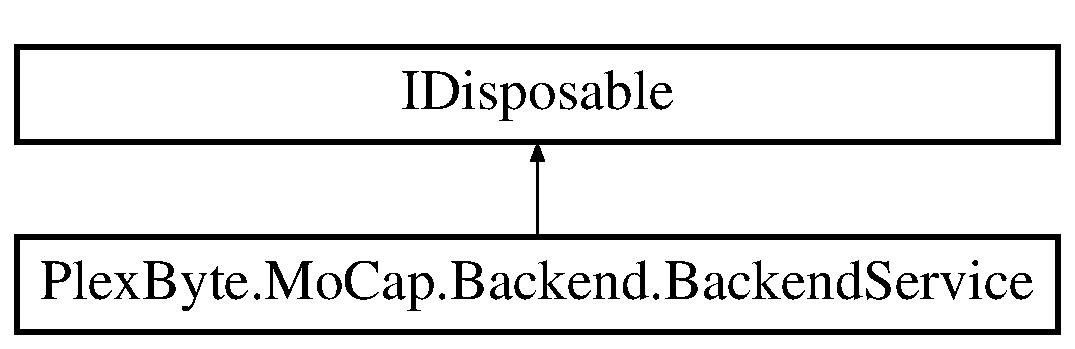
\includegraphics[height=2.000000cm]{class_plex_byte_1_1_mo_cap_1_1_backend_1_1_backend_service}
\end{center}
\end{figure}
\subsection*{Public Member Functions}
\begin{DoxyCompactItemize}
\item 
\hyperlink{class_plex_byte_1_1_mo_cap_1_1_backend_1_1_backend_service_a6515e3116617dbf054be2f26cd7b2e38}{Backend\+Service} ()
\item 
void \hyperlink{class_plex_byte_1_1_mo_cap_1_1_backend_1_1_backend_service_a7859887daa5e4bb760dedcbcc6fb7bf1}{Dispose} ()
\item 
Data\+Table \hyperlink{class_plex_byte_1_1_mo_cap_1_1_backend_1_1_backend_service_a1d64ef21282345f37aa3f42cba3656d2}{Authenticate\+User} (string p\+User\+Name, string p\+Password)
\begin{DoxyCompactList}\small\item\em This method authenticates the given user and password against the database. If suceeded the ID of the authenticated user will be returnes \end{DoxyCompactList}\item 
Date\+Time \hyperlink{class_plex_byte_1_1_mo_cap_1_1_backend_1_1_backend_service_ada231807a0c0116efff3a13c8d7fed3b}{Last\+User\+Login} (string p\+User\+Id)
\item 
Data\+Table \hyperlink{class_plex_byte_1_1_mo_cap_1_1_backend_1_1_backend_service_abe9eb812c39fcf5b1dd130ad3b0878b9}{Get\+Project\+By\+Id} (string p\+Id)
\item 
Data\+Table \hyperlink{class_plex_byte_1_1_mo_cap_1_1_backend_1_1_backend_service_ade6c8104facb7205953d0386b4119298}{Get\+Task\+By\+Id} (string p\+Id)
\item 
Data\+Table \hyperlink{class_plex_byte_1_1_mo_cap_1_1_backend_1_1_backend_service_a28c34c1d41ab5cc143ccfd5012481dfd}{Get\+Survey\+By\+Id} (string p\+Id)
\item 
Data\+Table \hyperlink{class_plex_byte_1_1_mo_cap_1_1_backend_1_1_backend_service_ae6b7cdf41f348ce844dfa08a876495c8}{Get\+Expense\+By\+Id} (string p\+Id)
\item 
Data\+Table \hyperlink{class_plex_byte_1_1_mo_cap_1_1_backend_1_1_backend_service_a01c6f0ba7587e8629b9ede895313ff76}{Get\+Timeslice\+By\+Id} (string p\+Id)
\item 
Data\+Table \hyperlink{class_plex_byte_1_1_mo_cap_1_1_backend_1_1_backend_service_aafab3576b46106ef63b5cc279e2f64bb}{Ge\+Survey\+Option\+By\+Id} (string p\+Id)
\item 
Data\+Table \hyperlink{class_plex_byte_1_1_mo_cap_1_1_backend_1_1_backend_service_ae70783055b16533fcfee00f2ba93469d}{Get\+Vote\+By\+Id} (string p\+Id, bool p\+Is\+Survey\+Id)
\begin{DoxyCompactList}\small\item\em This method returns either a single vote by its Id or a set of votes connected to a survey \end{DoxyCompactList}\item 
Data\+Table \hyperlink{class_plex_byte_1_1_mo_cap_1_1_backend_1_1_backend_service_a6d666dd173330adbf0b356f0144d398c}{Get\+User\+By\+Id} (string p\+Id)
\item 
Data\+Table \hyperlink{class_plex_byte_1_1_mo_cap_1_1_backend_1_1_backend_service_ad65376b62e58ba7139cfdb50f05ed929}{Get\+User\+By\+User\+Name} (string p\+User\+Name)
\item 
Data\+Table \hyperlink{class_plex_byte_1_1_mo_cap_1_1_backend_1_1_backend_service_a5e1cf727726998caf3fc700dc363b3bb}{Get\+User\+By\+Project\+Id} (string p\+Id)
\begin{DoxyCompactList}\small\item\em If project is the type, all users being member of the project with the Id specified will be returned. Otherwise the user with the Id given is returned \end{DoxyCompactList}\item 
Data\+Table \hyperlink{class_plex_byte_1_1_mo_cap_1_1_backend_1_1_backend_service_a30889d7e1506e065e2f88854fae1b120}{Get\+Task\+By\+Project\+Id} (string p\+Id)
\begin{DoxyCompactList}\small\item\em This method gets all task for the user\+Id or project\+Id specified and returns the datatable. \end{DoxyCompactList}\item 
Data\+Table \hyperlink{class_plex_byte_1_1_mo_cap_1_1_backend_1_1_backend_service_a21b1069392da4037e583f9d9fcad9d81}{Get\+Survey\+By\+Project\+Id} (string p\+Id, \hyperlink{namespace_plex_byte_1_1_mo_cap_1_1_backend_acbe18958b9ae9c08f5c2d2c580fbbf2a}{Object\+Type} p\+Type)
\begin{DoxyCompactList}\small\item\em This method gets all Surveys a user can participate in or were assigned to the project\+Id. \end{DoxyCompactList}\item 
Data\+Table \hyperlink{class_plex_byte_1_1_mo_cap_1_1_backend_1_1_backend_service_a0d49092e2ea8d8d1a6cad6fb0155906f}{Get\+Expense\+By\+Project\+Id} (string p\+Id, \hyperlink{namespace_plex_byte_1_1_mo_cap_1_1_backend_acbe18958b9ae9c08f5c2d2c580fbbf2a}{Object\+Type} p\+Type)
\begin{DoxyCompactList}\small\item\em This method gets all Expenses of a project. \end{DoxyCompactList}\item 
Data\+Table \hyperlink{class_plex_byte_1_1_mo_cap_1_1_backend_1_1_backend_service_a0ff59c331b4b94659b875602a54ece65}{Get\+Timeslice\+By\+Project\+Id} (string p\+Id, \hyperlink{namespace_plex_byte_1_1_mo_cap_1_1_backend_acbe18958b9ae9c08f5c2d2c580fbbf2a}{Object\+Type} p\+Type)
\begin{DoxyCompactList}\small\item\em This method gets all Timeslices of a project \end{DoxyCompactList}\item 
Data\+Table \hyperlink{class_plex_byte_1_1_mo_cap_1_1_backend_1_1_backend_service_a35fe823ccc300f00bd72f99313609835}{Get\+Survey\+Options} (string p\+Survey\+Id)
\begin{DoxyCompactList}\small\item\em This method gets all survey options that are available for the survey specified. It uses the S\+QL view\+\_\+surveyoptions \end{DoxyCompactList}\item 
Data\+Table \hyperlink{class_plex_byte_1_1_mo_cap_1_1_backend_1_1_backend_service_a709aa17c80b19ca328d99eb468b9054b}{Get\+Vote\+Count} (string p\+Survey\+Id)
\begin{DoxyCompactList}\small\item\em This method returns a recordset containing a grouped list of votes given for the survey id specified. It uses the S\+QL view\+\_\+votecount and has the following structure featuring a group by rollup \end{DoxyCompactList}\item 
Data\+Table \hyperlink{class_plex_byte_1_1_mo_cap_1_1_backend_1_1_backend_service_a922269b8f99a4c0c92d4d7df51f7024b}{Get\+Projects\+By\+User} (string p\+User\+Id)
\begin{DoxyCompactList}\small\item\em Returns all projects a user created, owns or is a member of \end{DoxyCompactList}\item 
Data\+Table \hyperlink{class_plex_byte_1_1_mo_cap_1_1_backend_1_1_backend_service_ab33310787b59934d0282f6f2d11d239c}{Get\+All\+Referenced\+Users} (string p\+User\+Id)
\item 
Data\+Table \hyperlink{class_plex_byte_1_1_mo_cap_1_1_backend_1_1_backend_service_a2f3b313c5d86880ca913320041b47d6a}{Get\+Expense\+By\+Project\+Id} (string p\+Id)
\begin{DoxyCompactList}\small\item\em This method returns all expenses for the user or project\+Id specified \end{DoxyCompactList}\item 
Data\+Table \hyperlink{class_plex_byte_1_1_mo_cap_1_1_backend_1_1_backend_service_aecab0686e55208dd16015580bc4082fc}{Get\+Time\+Slice\+By\+Project\+Id} (string p\+Id)
\begin{DoxyCompactList}\small\item\em This method returns all timeslices for the user or project\+Id specified \end{DoxyCompactList}\item 
Data\+Table \hyperlink{class_plex_byte_1_1_mo_cap_1_1_backend_1_1_backend_service_a84dac75b5ae2e9d807f9f617c652cfa0}{Get\+Account\+By\+Project\+Id} (string p\+Id)
\begin{DoxyCompactList}\small\item\em This method returns all users with Total\+Time and Total\+Value by project\+Id \end{DoxyCompactList}\item 
void \hyperlink{class_plex_byte_1_1_mo_cap_1_1_backend_1_1_backend_service_a3116d762269dad9511ad9be65b8bbc7a}{Insert\+User} (string p\+User\+Id, string p\+First\+Name, string p\+Last\+Name, string p\+Middle\+Name, string p\+Email, Date\+Time p\+Birthdate, string p\+User\+Name, string p\+Password)
\item 
void \hyperlink{class_plex_byte_1_1_mo_cap_1_1_backend_1_1_backend_service_af96d38adf2f202848701f9ca94148265}{Insert\+Project} (string p\+Project\+Id, string p\+Title, string p\+Description, Date\+Time p\+Start\+Date, Date\+Time p\+End\+Date, string p\+Owner, bool p\+Enable\+Balance, bool p\+Enable\+Survey, bool p\+Is\+Active, string p\+Creator, Enum p\+State\+Id)
\item 
void \hyperlink{class_plex_byte_1_1_mo_cap_1_1_backend_1_1_backend_service_afe6896f1ee35541cf824d5e44e58b013}{Insert\+Task} (string Task\+Id, string Interaction\+Id, Date\+Time Due\+Date\+Time, decimal Budget, int Duration, int Priority, int Progress, int Duration\+Used, decimal Budget\+Used, Date\+Time Start\+Date\+Time, Date\+Time End\+Date\+Time, bool Is\+Active, string Text, string Creator\+Id, string Owner\+Id, string State\+Id, string Project\+Id)
\item 
void \hyperlink{class_plex_byte_1_1_mo_cap_1_1_backend_1_1_backend_service_a0d1bc95f01b316823e1a45471f91ba85}{Insert\+Vote} (string p\+Survey\+Id, string p\+Option\+Id, string p\+User\+Id, Date\+Time p\+Created)
\item 
void \hyperlink{class_plex_byte_1_1_mo_cap_1_1_backend_1_1_backend_service_a81a6b7116d17a1d9dce39e5c8883cd0f}{Insert\+Survey} (string p\+Id, string p\+Interaction\+Id, int p\+Votes\+Per\+User, Date\+Time p\+Due\+Date\+Time, Date\+Time p\+Start\+Date\+Time, Date\+Time p\+End\+Date\+Time, string p\+Creator\+Id, string p\+Owner\+Id, bool p\+Is\+Active, Interaction\+State p\+State, string p\+Project\+Id, string p\+Text, string p\+Title)
\item 
void \hyperlink{class_plex_byte_1_1_mo_cap_1_1_backend_1_1_backend_service_a57d4da2ed2044f2f5bddc24ca92ee003}{Insert\+Survey\+Option} (string p\+Id, string p\+Text, string p\+Survey\+Id)
\item 
void \hyperlink{class_plex_byte_1_1_mo_cap_1_1_backend_1_1_backend_service_a69c06da763b493aceaeab04a43c41dab}{Insert\+Timeslice} (string p\+Id, int p\+Duration, string p\+Target\+Id, string p\+Description, string p\+Target\+Type, Date\+Time p\+Created\+Date\+Time)
\item 
void \hyperlink{class_plex_byte_1_1_mo_cap_1_1_backend_1_1_backend_service_acd4446e6836f11aa2df58262530a92a5}{Insert\+Project\+Mapping} (string Project\+Id, string Object\+Id, int \hyperlink{namespace_plex_byte_1_1_mo_cap_1_1_backend_acbe18958b9ae9c08f5c2d2c580fbbf2a}{Object\+Type})
\end{DoxyCompactItemize}


\subsection{Detailed Description}


Definition at line 25 of file Backend\+Service.\+cs.



\subsection{Constructor \& Destructor Documentation}
\index{Plex\+Byte\+::\+Mo\+Cap\+::\+Backend\+::\+Backend\+Service@{Plex\+Byte\+::\+Mo\+Cap\+::\+Backend\+::\+Backend\+Service}!Backend\+Service@{Backend\+Service}}
\index{Backend\+Service@{Backend\+Service}!Plex\+Byte\+::\+Mo\+Cap\+::\+Backend\+::\+Backend\+Service@{Plex\+Byte\+::\+Mo\+Cap\+::\+Backend\+::\+Backend\+Service}}
\subsubsection[{\texorpdfstring{Backend\+Service()}{BackendService()}}]{\setlength{\rightskip}{0pt plus 5cm}Plex\+Byte.\+Mo\+Cap.\+Backend.\+Backend\+Service.\+Backend\+Service (
\begin{DoxyParamCaption}
{}
\end{DoxyParamCaption}
)}\hypertarget{class_plex_byte_1_1_mo_cap_1_1_backend_1_1_backend_service_a6515e3116617dbf054be2f26cd7b2e38}{}\label{class_plex_byte_1_1_mo_cap_1_1_backend_1_1_backend_service_a6515e3116617dbf054be2f26cd7b2e38}


Definition at line 33 of file Backend\+Service.\+cs.



\subsection{Member Function Documentation}
\index{Plex\+Byte\+::\+Mo\+Cap\+::\+Backend\+::\+Backend\+Service@{Plex\+Byte\+::\+Mo\+Cap\+::\+Backend\+::\+Backend\+Service}!Authenticate\+User@{Authenticate\+User}}
\index{Authenticate\+User@{Authenticate\+User}!Plex\+Byte\+::\+Mo\+Cap\+::\+Backend\+::\+Backend\+Service@{Plex\+Byte\+::\+Mo\+Cap\+::\+Backend\+::\+Backend\+Service}}
\subsubsection[{\texorpdfstring{Authenticate\+User(string p\+User\+Name, string p\+Password)}{AuthenticateUser(string pUserName, string pPassword)}}]{\setlength{\rightskip}{0pt plus 5cm}Data\+Table Plex\+Byte.\+Mo\+Cap.\+Backend.\+Backend\+Service.\+Authenticate\+User (
\begin{DoxyParamCaption}
\item[{string}]{p\+User\+Name, }
\item[{string}]{p\+Password}
\end{DoxyParamCaption}
)}\hypertarget{class_plex_byte_1_1_mo_cap_1_1_backend_1_1_backend_service_a1d64ef21282345f37aa3f42cba3656d2}{}\label{class_plex_byte_1_1_mo_cap_1_1_backend_1_1_backend_service_a1d64ef21282345f37aa3f42cba3656d2}


This method authenticates the given user and password against the database. If suceeded the ID of the authenticated user will be returnes 


\begin{DoxyParams}{Parameters}
{\em p\+Id} & The id of the user to query results for\\
\hline
\end{DoxyParams}
\begin{DoxyReturn}{Returns}
The Users Id
\end{DoxyReturn}


Definition at line 45 of file Backend\+Service.\+cs.

\index{Plex\+Byte\+::\+Mo\+Cap\+::\+Backend\+::\+Backend\+Service@{Plex\+Byte\+::\+Mo\+Cap\+::\+Backend\+::\+Backend\+Service}!Dispose@{Dispose}}
\index{Dispose@{Dispose}!Plex\+Byte\+::\+Mo\+Cap\+::\+Backend\+::\+Backend\+Service@{Plex\+Byte\+::\+Mo\+Cap\+::\+Backend\+::\+Backend\+Service}}
\subsubsection[{\texorpdfstring{Dispose()}{Dispose()}}]{\setlength{\rightskip}{0pt plus 5cm}void Plex\+Byte.\+Mo\+Cap.\+Backend.\+Backend\+Service.\+Dispose (
\begin{DoxyParamCaption}
{}
\end{DoxyParamCaption}
)}\hypertarget{class_plex_byte_1_1_mo_cap_1_1_backend_1_1_backend_service_a7859887daa5e4bb760dedcbcc6fb7bf1}{}\label{class_plex_byte_1_1_mo_cap_1_1_backend_1_1_backend_service_a7859887daa5e4bb760dedcbcc6fb7bf1}


Definition at line 38 of file Backend\+Service.\+cs.

\index{Plex\+Byte\+::\+Mo\+Cap\+::\+Backend\+::\+Backend\+Service@{Plex\+Byte\+::\+Mo\+Cap\+::\+Backend\+::\+Backend\+Service}!Ge\+Survey\+Option\+By\+Id@{Ge\+Survey\+Option\+By\+Id}}
\index{Ge\+Survey\+Option\+By\+Id@{Ge\+Survey\+Option\+By\+Id}!Plex\+Byte\+::\+Mo\+Cap\+::\+Backend\+::\+Backend\+Service@{Plex\+Byte\+::\+Mo\+Cap\+::\+Backend\+::\+Backend\+Service}}
\subsubsection[{\texorpdfstring{Ge\+Survey\+Option\+By\+Id(string p\+Id)}{GeSurveyOptionById(string pId)}}]{\setlength{\rightskip}{0pt plus 5cm}Data\+Table Plex\+Byte.\+Mo\+Cap.\+Backend.\+Backend\+Service.\+Ge\+Survey\+Option\+By\+Id (
\begin{DoxyParamCaption}
\item[{string}]{p\+Id}
\end{DoxyParamCaption}
)}\hypertarget{class_plex_byte_1_1_mo_cap_1_1_backend_1_1_backend_service_aafab3576b46106ef63b5cc279e2f64bb}{}\label{class_plex_byte_1_1_mo_cap_1_1_backend_1_1_backend_service_aafab3576b46106ef63b5cc279e2f64bb}


Definition at line 127 of file Backend\+Service.\+cs.

\index{Plex\+Byte\+::\+Mo\+Cap\+::\+Backend\+::\+Backend\+Service@{Plex\+Byte\+::\+Mo\+Cap\+::\+Backend\+::\+Backend\+Service}!Get\+Account\+By\+Project\+Id@{Get\+Account\+By\+Project\+Id}}
\index{Get\+Account\+By\+Project\+Id@{Get\+Account\+By\+Project\+Id}!Plex\+Byte\+::\+Mo\+Cap\+::\+Backend\+::\+Backend\+Service@{Plex\+Byte\+::\+Mo\+Cap\+::\+Backend\+::\+Backend\+Service}}
\subsubsection[{\texorpdfstring{Get\+Account\+By\+Project\+Id(string p\+Id)}{GetAccountByProjectId(string pId)}}]{\setlength{\rightskip}{0pt plus 5cm}Data\+Table Plex\+Byte.\+Mo\+Cap.\+Backend.\+Backend\+Service.\+Get\+Account\+By\+Project\+Id (
\begin{DoxyParamCaption}
\item[{string}]{p\+Id}
\end{DoxyParamCaption}
)}\hypertarget{class_plex_byte_1_1_mo_cap_1_1_backend_1_1_backend_service_a84dac75b5ae2e9d807f9f617c652cfa0}{}\label{class_plex_byte_1_1_mo_cap_1_1_backend_1_1_backend_service_a84dac75b5ae2e9d807f9f617c652cfa0}


This method returns all users with Total\+Time and Total\+Value by project\+Id 


\begin{DoxyParams}{Parameters}
{\em p\+Id} & \\
\hline
\end{DoxyParams}
\begin{DoxyReturn}{Returns}
Data\+Table with\+: \mbox{[}p\mbox{]}.\mbox{[}Id\mbox{]} AS Project\+Id, \mbox{[}p\mbox{]}.\mbox{[}Name\mbox{]}, \mbox{[}u\mbox{]}.\mbox{[}Id\mbox{]} AS User\+Id, \mbox{[}u\mbox{]}.\mbox{[}Username\mbox{]}, S\+UM(\mbox{[}t\mbox{]}.\mbox{[}Duration\mbox{]}) AS Total\+Time, S\+UM(\mbox{[}e\mbox{]}.\mbox{[}Value\mbox{]}) AS Total\+Value, \mbox{[}p\mbox{]}.\mbox{[}Is\+Active\mbox{]}
\end{DoxyReturn}


Definition at line 317 of file Backend\+Service.\+cs.

\index{Plex\+Byte\+::\+Mo\+Cap\+::\+Backend\+::\+Backend\+Service@{Plex\+Byte\+::\+Mo\+Cap\+::\+Backend\+::\+Backend\+Service}!Get\+All\+Referenced\+Users@{Get\+All\+Referenced\+Users}}
\index{Get\+All\+Referenced\+Users@{Get\+All\+Referenced\+Users}!Plex\+Byte\+::\+Mo\+Cap\+::\+Backend\+::\+Backend\+Service@{Plex\+Byte\+::\+Mo\+Cap\+::\+Backend\+::\+Backend\+Service}}
\subsubsection[{\texorpdfstring{Get\+All\+Referenced\+Users(string p\+User\+Id)}{GetAllReferencedUsers(string pUserId)}}]{\setlength{\rightskip}{0pt plus 5cm}Data\+Table Plex\+Byte.\+Mo\+Cap.\+Backend.\+Backend\+Service.\+Get\+All\+Referenced\+Users (
\begin{DoxyParamCaption}
\item[{string}]{p\+User\+Id}
\end{DoxyParamCaption}
)}\hypertarget{class_plex_byte_1_1_mo_cap_1_1_backend_1_1_backend_service_ab33310787b59934d0282f6f2d11d239c}{}\label{class_plex_byte_1_1_mo_cap_1_1_backend_1_1_backend_service_ab33310787b59934d0282f6f2d11d239c}


Definition at line 269 of file Backend\+Service.\+cs.

\index{Plex\+Byte\+::\+Mo\+Cap\+::\+Backend\+::\+Backend\+Service@{Plex\+Byte\+::\+Mo\+Cap\+::\+Backend\+::\+Backend\+Service}!Get\+Expense\+By\+Id@{Get\+Expense\+By\+Id}}
\index{Get\+Expense\+By\+Id@{Get\+Expense\+By\+Id}!Plex\+Byte\+::\+Mo\+Cap\+::\+Backend\+::\+Backend\+Service@{Plex\+Byte\+::\+Mo\+Cap\+::\+Backend\+::\+Backend\+Service}}
\subsubsection[{\texorpdfstring{Get\+Expense\+By\+Id(string p\+Id)}{GetExpenseById(string pId)}}]{\setlength{\rightskip}{0pt plus 5cm}Data\+Table Plex\+Byte.\+Mo\+Cap.\+Backend.\+Backend\+Service.\+Get\+Expense\+By\+Id (
\begin{DoxyParamCaption}
\item[{string}]{p\+Id}
\end{DoxyParamCaption}
)}\hypertarget{class_plex_byte_1_1_mo_cap_1_1_backend_1_1_backend_service_ae6b7cdf41f348ce844dfa08a876495c8}{}\label{class_plex_byte_1_1_mo_cap_1_1_backend_1_1_backend_service_ae6b7cdf41f348ce844dfa08a876495c8}


Definition at line 117 of file Backend\+Service.\+cs.

\index{Plex\+Byte\+::\+Mo\+Cap\+::\+Backend\+::\+Backend\+Service@{Plex\+Byte\+::\+Mo\+Cap\+::\+Backend\+::\+Backend\+Service}!Get\+Expense\+By\+Project\+Id@{Get\+Expense\+By\+Project\+Id}}
\index{Get\+Expense\+By\+Project\+Id@{Get\+Expense\+By\+Project\+Id}!Plex\+Byte\+::\+Mo\+Cap\+::\+Backend\+::\+Backend\+Service@{Plex\+Byte\+::\+Mo\+Cap\+::\+Backend\+::\+Backend\+Service}}
\subsubsection[{\texorpdfstring{Get\+Expense\+By\+Project\+Id(string p\+Id, Object\+Type p\+Type)}{GetExpenseByProjectId(string pId, ObjectType pType)}}]{\setlength{\rightskip}{0pt plus 5cm}Data\+Table Plex\+Byte.\+Mo\+Cap.\+Backend.\+Backend\+Service.\+Get\+Expense\+By\+Project\+Id (
\begin{DoxyParamCaption}
\item[{string}]{p\+Id, }
\item[{{\bf Object\+Type}}]{p\+Type}
\end{DoxyParamCaption}
)}\hypertarget{class_plex_byte_1_1_mo_cap_1_1_backend_1_1_backend_service_a0d49092e2ea8d8d1a6cad6fb0155906f}{}\label{class_plex_byte_1_1_mo_cap_1_1_backend_1_1_backend_service_a0d49092e2ea8d8d1a6cad6fb0155906f}


This method gets all Expenses of a project. 


\begin{DoxyParams}{Parameters}
{\em p\+Id} & The id of the project to query\\
\hline
{\em p\+Type} & The object type to use in the query (either Project or User)\\
\hline
\end{DoxyParams}
\begin{DoxyReturn}{Returns}
Data\+Table containing all Expenses for the user or project in question
\end{DoxyReturn}


Definition at line 204 of file Backend\+Service.\+cs.

\index{Plex\+Byte\+::\+Mo\+Cap\+::\+Backend\+::\+Backend\+Service@{Plex\+Byte\+::\+Mo\+Cap\+::\+Backend\+::\+Backend\+Service}!Get\+Expense\+By\+Project\+Id@{Get\+Expense\+By\+Project\+Id}}
\index{Get\+Expense\+By\+Project\+Id@{Get\+Expense\+By\+Project\+Id}!Plex\+Byte\+::\+Mo\+Cap\+::\+Backend\+::\+Backend\+Service@{Plex\+Byte\+::\+Mo\+Cap\+::\+Backend\+::\+Backend\+Service}}
\subsubsection[{\texorpdfstring{Get\+Expense\+By\+Project\+Id(string p\+Id)}{GetExpenseByProjectId(string pId)}}]{\setlength{\rightskip}{0pt plus 5cm}Data\+Table Plex\+Byte.\+Mo\+Cap.\+Backend.\+Backend\+Service.\+Get\+Expense\+By\+Project\+Id (
\begin{DoxyParamCaption}
\item[{string}]{p\+Id}
\end{DoxyParamCaption}
)}\hypertarget{class_plex_byte_1_1_mo_cap_1_1_backend_1_1_backend_service_a2f3b313c5d86880ca913320041b47d6a}{}\label{class_plex_byte_1_1_mo_cap_1_1_backend_1_1_backend_service_a2f3b313c5d86880ca913320041b47d6a}


This method returns all expenses for the user or project\+Id specified 


\begin{DoxyParams}{Parameters}
{\em p\+Id} & The id to use in the query\\
\hline
{\em p\+Type} & The object type to use in the query (either Project or User)\\
\hline
\end{DoxyParams}
\begin{DoxyReturn}{Returns}
Data\+Table containing all expenses
\end{DoxyReturn}


Definition at line 294 of file Backend\+Service.\+cs.

\index{Plex\+Byte\+::\+Mo\+Cap\+::\+Backend\+::\+Backend\+Service@{Plex\+Byte\+::\+Mo\+Cap\+::\+Backend\+::\+Backend\+Service}!Get\+Project\+By\+Id@{Get\+Project\+By\+Id}}
\index{Get\+Project\+By\+Id@{Get\+Project\+By\+Id}!Plex\+Byte\+::\+Mo\+Cap\+::\+Backend\+::\+Backend\+Service@{Plex\+Byte\+::\+Mo\+Cap\+::\+Backend\+::\+Backend\+Service}}
\subsubsection[{\texorpdfstring{Get\+Project\+By\+Id(string p\+Id)}{GetProjectById(string pId)}}]{\setlength{\rightskip}{0pt plus 5cm}Data\+Table Plex\+Byte.\+Mo\+Cap.\+Backend.\+Backend\+Service.\+Get\+Project\+By\+Id (
\begin{DoxyParamCaption}
\item[{string}]{p\+Id}
\end{DoxyParamCaption}
)}\hypertarget{class_plex_byte_1_1_mo_cap_1_1_backend_1_1_backend_service_abe9eb812c39fcf5b1dd130ad3b0878b9}{}\label{class_plex_byte_1_1_mo_cap_1_1_backend_1_1_backend_service_abe9eb812c39fcf5b1dd130ad3b0878b9}


Definition at line 102 of file Backend\+Service.\+cs.

\index{Plex\+Byte\+::\+Mo\+Cap\+::\+Backend\+::\+Backend\+Service@{Plex\+Byte\+::\+Mo\+Cap\+::\+Backend\+::\+Backend\+Service}!Get\+Projects\+By\+User@{Get\+Projects\+By\+User}}
\index{Get\+Projects\+By\+User@{Get\+Projects\+By\+User}!Plex\+Byte\+::\+Mo\+Cap\+::\+Backend\+::\+Backend\+Service@{Plex\+Byte\+::\+Mo\+Cap\+::\+Backend\+::\+Backend\+Service}}
\subsubsection[{\texorpdfstring{Get\+Projects\+By\+User(string p\+User\+Id)}{GetProjectsByUser(string pUserId)}}]{\setlength{\rightskip}{0pt plus 5cm}Data\+Table Plex\+Byte.\+Mo\+Cap.\+Backend.\+Backend\+Service.\+Get\+Projects\+By\+User (
\begin{DoxyParamCaption}
\item[{string}]{p\+User\+Id}
\end{DoxyParamCaption}
)}\hypertarget{class_plex_byte_1_1_mo_cap_1_1_backend_1_1_backend_service_a922269b8f99a4c0c92d4d7df51f7024b}{}\label{class_plex_byte_1_1_mo_cap_1_1_backend_1_1_backend_service_a922269b8f99a4c0c92d4d7df51f7024b}


Returns all projects a user created, owns or is a member of 


\begin{DoxyParams}{Parameters}
{\em p\+User\+Id} & The user Id to use in the query\\
\hline
\end{DoxyParams}
\begin{DoxyReturn}{Returns}
Data\+Set containing all projects for this user
\end{DoxyReturn}


Definition at line 262 of file Backend\+Service.\+cs.

\index{Plex\+Byte\+::\+Mo\+Cap\+::\+Backend\+::\+Backend\+Service@{Plex\+Byte\+::\+Mo\+Cap\+::\+Backend\+::\+Backend\+Service}!Get\+Survey\+By\+Id@{Get\+Survey\+By\+Id}}
\index{Get\+Survey\+By\+Id@{Get\+Survey\+By\+Id}!Plex\+Byte\+::\+Mo\+Cap\+::\+Backend\+::\+Backend\+Service@{Plex\+Byte\+::\+Mo\+Cap\+::\+Backend\+::\+Backend\+Service}}
\subsubsection[{\texorpdfstring{Get\+Survey\+By\+Id(string p\+Id)}{GetSurveyById(string pId)}}]{\setlength{\rightskip}{0pt plus 5cm}Data\+Table Plex\+Byte.\+Mo\+Cap.\+Backend.\+Backend\+Service.\+Get\+Survey\+By\+Id (
\begin{DoxyParamCaption}
\item[{string}]{p\+Id}
\end{DoxyParamCaption}
)}\hypertarget{class_plex_byte_1_1_mo_cap_1_1_backend_1_1_backend_service_a28c34c1d41ab5cc143ccfd5012481dfd}{}\label{class_plex_byte_1_1_mo_cap_1_1_backend_1_1_backend_service_a28c34c1d41ab5cc143ccfd5012481dfd}


Definition at line 112 of file Backend\+Service.\+cs.

\index{Plex\+Byte\+::\+Mo\+Cap\+::\+Backend\+::\+Backend\+Service@{Plex\+Byte\+::\+Mo\+Cap\+::\+Backend\+::\+Backend\+Service}!Get\+Survey\+By\+Project\+Id@{Get\+Survey\+By\+Project\+Id}}
\index{Get\+Survey\+By\+Project\+Id@{Get\+Survey\+By\+Project\+Id}!Plex\+Byte\+::\+Mo\+Cap\+::\+Backend\+::\+Backend\+Service@{Plex\+Byte\+::\+Mo\+Cap\+::\+Backend\+::\+Backend\+Service}}
\subsubsection[{\texorpdfstring{Get\+Survey\+By\+Project\+Id(string p\+Id, Object\+Type p\+Type)}{GetSurveyByProjectId(string pId, ObjectType pType)}}]{\setlength{\rightskip}{0pt plus 5cm}Data\+Table Plex\+Byte.\+Mo\+Cap.\+Backend.\+Backend\+Service.\+Get\+Survey\+By\+Project\+Id (
\begin{DoxyParamCaption}
\item[{string}]{p\+Id, }
\item[{{\bf Object\+Type}}]{p\+Type}
\end{DoxyParamCaption}
)}\hypertarget{class_plex_byte_1_1_mo_cap_1_1_backend_1_1_backend_service_a21b1069392da4037e583f9d9fcad9d81}{}\label{class_plex_byte_1_1_mo_cap_1_1_backend_1_1_backend_service_a21b1069392da4037e583f9d9fcad9d81}


This method gets all Surveys a user can participate in or were assigned to the project\+Id. 


\begin{DoxyParams}{Parameters}
{\em p\+Id} & The id of the user or project to query\\
\hline
{\em p\+Type} & The object type to use in the query (either Project or User)\\
\hline
\end{DoxyParams}
\begin{DoxyReturn}{Returns}
Data\+Table containing all Survey for the user or project in question
\end{DoxyReturn}


Definition at line 191 of file Backend\+Service.\+cs.

\index{Plex\+Byte\+::\+Mo\+Cap\+::\+Backend\+::\+Backend\+Service@{Plex\+Byte\+::\+Mo\+Cap\+::\+Backend\+::\+Backend\+Service}!Get\+Survey\+Options@{Get\+Survey\+Options}}
\index{Get\+Survey\+Options@{Get\+Survey\+Options}!Plex\+Byte\+::\+Mo\+Cap\+::\+Backend\+::\+Backend\+Service@{Plex\+Byte\+::\+Mo\+Cap\+::\+Backend\+::\+Backend\+Service}}
\subsubsection[{\texorpdfstring{Get\+Survey\+Options(string p\+Survey\+Id)}{GetSurveyOptions(string pSurveyId)}}]{\setlength{\rightskip}{0pt plus 5cm}Data\+Table Plex\+Byte.\+Mo\+Cap.\+Backend.\+Backend\+Service.\+Get\+Survey\+Options (
\begin{DoxyParamCaption}
\item[{string}]{p\+Survey\+Id}
\end{DoxyParamCaption}
)}\hypertarget{class_plex_byte_1_1_mo_cap_1_1_backend_1_1_backend_service_a35fe823ccc300f00bd72f99313609835}{}\label{class_plex_byte_1_1_mo_cap_1_1_backend_1_1_backend_service_a35fe823ccc300f00bd72f99313609835}


This method gets all survey options that are available for the survey specified. It uses the S\+QL view\+\_\+surveyoptions 


\begin{DoxyParams}{Parameters}
{\em p\+Survey\+Id} & The id of the survey to query\\
\hline
\end{DoxyParams}
\begin{DoxyReturn}{Returns}
Data\+Table containing all Survey Options for the Survey in question
\end{DoxyReturn}


Definition at line 226 of file Backend\+Service.\+cs.

\index{Plex\+Byte\+::\+Mo\+Cap\+::\+Backend\+::\+Backend\+Service@{Plex\+Byte\+::\+Mo\+Cap\+::\+Backend\+::\+Backend\+Service}!Get\+Task\+By\+Id@{Get\+Task\+By\+Id}}
\index{Get\+Task\+By\+Id@{Get\+Task\+By\+Id}!Plex\+Byte\+::\+Mo\+Cap\+::\+Backend\+::\+Backend\+Service@{Plex\+Byte\+::\+Mo\+Cap\+::\+Backend\+::\+Backend\+Service}}
\subsubsection[{\texorpdfstring{Get\+Task\+By\+Id(string p\+Id)}{GetTaskById(string pId)}}]{\setlength{\rightskip}{0pt plus 5cm}Data\+Table Plex\+Byte.\+Mo\+Cap.\+Backend.\+Backend\+Service.\+Get\+Task\+By\+Id (
\begin{DoxyParamCaption}
\item[{string}]{p\+Id}
\end{DoxyParamCaption}
)}\hypertarget{class_plex_byte_1_1_mo_cap_1_1_backend_1_1_backend_service_ade6c8104facb7205953d0386b4119298}{}\label{class_plex_byte_1_1_mo_cap_1_1_backend_1_1_backend_service_ade6c8104facb7205953d0386b4119298}


Definition at line 107 of file Backend\+Service.\+cs.

\index{Plex\+Byte\+::\+Mo\+Cap\+::\+Backend\+::\+Backend\+Service@{Plex\+Byte\+::\+Mo\+Cap\+::\+Backend\+::\+Backend\+Service}!Get\+Task\+By\+Project\+Id@{Get\+Task\+By\+Project\+Id}}
\index{Get\+Task\+By\+Project\+Id@{Get\+Task\+By\+Project\+Id}!Plex\+Byte\+::\+Mo\+Cap\+::\+Backend\+::\+Backend\+Service@{Plex\+Byte\+::\+Mo\+Cap\+::\+Backend\+::\+Backend\+Service}}
\subsubsection[{\texorpdfstring{Get\+Task\+By\+Project\+Id(string p\+Id)}{GetTaskByProjectId(string pId)}}]{\setlength{\rightskip}{0pt plus 5cm}Data\+Table Plex\+Byte.\+Mo\+Cap.\+Backend.\+Backend\+Service.\+Get\+Task\+By\+Project\+Id (
\begin{DoxyParamCaption}
\item[{string}]{p\+Id}
\end{DoxyParamCaption}
)}\hypertarget{class_plex_byte_1_1_mo_cap_1_1_backend_1_1_backend_service_a30889d7e1506e065e2f88854fae1b120}{}\label{class_plex_byte_1_1_mo_cap_1_1_backend_1_1_backend_service_a30889d7e1506e065e2f88854fae1b120}


This method gets all task for the user\+Id or project\+Id specified and returns the datatable. 


\begin{DoxyParams}{Parameters}
{\em p\+Id} & The id of the user or project to query\\
\hline
{\em p\+Type} & The object type to use in the query (either Project or User)\\
\hline
\end{DoxyParams}
\begin{DoxyReturn}{Returns}
Data\+Table containing all tasks for the user or project in question
\end{DoxyReturn}


Definition at line 180 of file Backend\+Service.\+cs.

\index{Plex\+Byte\+::\+Mo\+Cap\+::\+Backend\+::\+Backend\+Service@{Plex\+Byte\+::\+Mo\+Cap\+::\+Backend\+::\+Backend\+Service}!Get\+Timeslice\+By\+Id@{Get\+Timeslice\+By\+Id}}
\index{Get\+Timeslice\+By\+Id@{Get\+Timeslice\+By\+Id}!Plex\+Byte\+::\+Mo\+Cap\+::\+Backend\+::\+Backend\+Service@{Plex\+Byte\+::\+Mo\+Cap\+::\+Backend\+::\+Backend\+Service}}
\subsubsection[{\texorpdfstring{Get\+Timeslice\+By\+Id(string p\+Id)}{GetTimesliceById(string pId)}}]{\setlength{\rightskip}{0pt plus 5cm}Data\+Table Plex\+Byte.\+Mo\+Cap.\+Backend.\+Backend\+Service.\+Get\+Timeslice\+By\+Id (
\begin{DoxyParamCaption}
\item[{string}]{p\+Id}
\end{DoxyParamCaption}
)}\hypertarget{class_plex_byte_1_1_mo_cap_1_1_backend_1_1_backend_service_a01c6f0ba7587e8629b9ede895313ff76}{}\label{class_plex_byte_1_1_mo_cap_1_1_backend_1_1_backend_service_a01c6f0ba7587e8629b9ede895313ff76}


Definition at line 122 of file Backend\+Service.\+cs.

\index{Plex\+Byte\+::\+Mo\+Cap\+::\+Backend\+::\+Backend\+Service@{Plex\+Byte\+::\+Mo\+Cap\+::\+Backend\+::\+Backend\+Service}!Get\+Timeslice\+By\+Project\+Id@{Get\+Timeslice\+By\+Project\+Id}}
\index{Get\+Timeslice\+By\+Project\+Id@{Get\+Timeslice\+By\+Project\+Id}!Plex\+Byte\+::\+Mo\+Cap\+::\+Backend\+::\+Backend\+Service@{Plex\+Byte\+::\+Mo\+Cap\+::\+Backend\+::\+Backend\+Service}}
\subsubsection[{\texorpdfstring{Get\+Timeslice\+By\+Project\+Id(string p\+Id, Object\+Type p\+Type)}{GetTimesliceByProjectId(string pId, ObjectType pType)}}]{\setlength{\rightskip}{0pt plus 5cm}Data\+Table Plex\+Byte.\+Mo\+Cap.\+Backend.\+Backend\+Service.\+Get\+Timeslice\+By\+Project\+Id (
\begin{DoxyParamCaption}
\item[{string}]{p\+Id, }
\item[{{\bf Object\+Type}}]{p\+Type}
\end{DoxyParamCaption}
)}\hypertarget{class_plex_byte_1_1_mo_cap_1_1_backend_1_1_backend_service_a0ff59c331b4b94659b875602a54ece65}{}\label{class_plex_byte_1_1_mo_cap_1_1_backend_1_1_backend_service_a0ff59c331b4b94659b875602a54ece65}


This method gets all Timeslices of a project 


\begin{DoxyParams}{Parameters}
{\em p\+Id} & The id of the project to query\\
\hline
{\em p\+Type} & The object type to use in the query (either Project or User)\\
\hline
\end{DoxyParams}
\begin{DoxyReturn}{Returns}
Data\+Table containing all Timeslices for the user or project in question
\end{DoxyReturn}


Definition at line 216 of file Backend\+Service.\+cs.

\index{Plex\+Byte\+::\+Mo\+Cap\+::\+Backend\+::\+Backend\+Service@{Plex\+Byte\+::\+Mo\+Cap\+::\+Backend\+::\+Backend\+Service}!Get\+Time\+Slice\+By\+Project\+Id@{Get\+Time\+Slice\+By\+Project\+Id}}
\index{Get\+Time\+Slice\+By\+Project\+Id@{Get\+Time\+Slice\+By\+Project\+Id}!Plex\+Byte\+::\+Mo\+Cap\+::\+Backend\+::\+Backend\+Service@{Plex\+Byte\+::\+Mo\+Cap\+::\+Backend\+::\+Backend\+Service}}
\subsubsection[{\texorpdfstring{Get\+Time\+Slice\+By\+Project\+Id(string p\+Id)}{GetTimeSliceByProjectId(string pId)}}]{\setlength{\rightskip}{0pt plus 5cm}Data\+Table Plex\+Byte.\+Mo\+Cap.\+Backend.\+Backend\+Service.\+Get\+Time\+Slice\+By\+Project\+Id (
\begin{DoxyParamCaption}
\item[{string}]{p\+Id}
\end{DoxyParamCaption}
)}\hypertarget{class_plex_byte_1_1_mo_cap_1_1_backend_1_1_backend_service_aecab0686e55208dd16015580bc4082fc}{}\label{class_plex_byte_1_1_mo_cap_1_1_backend_1_1_backend_service_aecab0686e55208dd16015580bc4082fc}


This method returns all timeslices for the user or project\+Id specified 


\begin{DoxyParams}{Parameters}
{\em p\+Id} & The id to use in the query\\
\hline
{\em p\+Type} & The object type to use in the query (either Project or User)\\
\hline
\end{DoxyParams}
\begin{DoxyReturn}{Returns}
Data\+Table containing all timeslices


\end{DoxyReturn}


Definition at line 306 of file Backend\+Service.\+cs.

\index{Plex\+Byte\+::\+Mo\+Cap\+::\+Backend\+::\+Backend\+Service@{Plex\+Byte\+::\+Mo\+Cap\+::\+Backend\+::\+Backend\+Service}!Get\+User\+By\+Id@{Get\+User\+By\+Id}}
\index{Get\+User\+By\+Id@{Get\+User\+By\+Id}!Plex\+Byte\+::\+Mo\+Cap\+::\+Backend\+::\+Backend\+Service@{Plex\+Byte\+::\+Mo\+Cap\+::\+Backend\+::\+Backend\+Service}}
\subsubsection[{\texorpdfstring{Get\+User\+By\+Id(string p\+Id)}{GetUserById(string pId)}}]{\setlength{\rightskip}{0pt plus 5cm}Data\+Table Plex\+Byte.\+Mo\+Cap.\+Backend.\+Backend\+Service.\+Get\+User\+By\+Id (
\begin{DoxyParamCaption}
\item[{string}]{p\+Id}
\end{DoxyParamCaption}
)}\hypertarget{class_plex_byte_1_1_mo_cap_1_1_backend_1_1_backend_service_a6d666dd173330adbf0b356f0144d398c}{}\label{class_plex_byte_1_1_mo_cap_1_1_backend_1_1_backend_service_a6d666dd173330adbf0b356f0144d398c}


Definition at line 152 of file Backend\+Service.\+cs.

\index{Plex\+Byte\+::\+Mo\+Cap\+::\+Backend\+::\+Backend\+Service@{Plex\+Byte\+::\+Mo\+Cap\+::\+Backend\+::\+Backend\+Service}!Get\+User\+By\+Project\+Id@{Get\+User\+By\+Project\+Id}}
\index{Get\+User\+By\+Project\+Id@{Get\+User\+By\+Project\+Id}!Plex\+Byte\+::\+Mo\+Cap\+::\+Backend\+::\+Backend\+Service@{Plex\+Byte\+::\+Mo\+Cap\+::\+Backend\+::\+Backend\+Service}}
\subsubsection[{\texorpdfstring{Get\+User\+By\+Project\+Id(string p\+Id)}{GetUserByProjectId(string pId)}}]{\setlength{\rightskip}{0pt plus 5cm}Data\+Table Plex\+Byte.\+Mo\+Cap.\+Backend.\+Backend\+Service.\+Get\+User\+By\+Project\+Id (
\begin{DoxyParamCaption}
\item[{string}]{p\+Id}
\end{DoxyParamCaption}
)}\hypertarget{class_plex_byte_1_1_mo_cap_1_1_backend_1_1_backend_service_a5e1cf727726998caf3fc700dc363b3bb}{}\label{class_plex_byte_1_1_mo_cap_1_1_backend_1_1_backend_service_a5e1cf727726998caf3fc700dc363b3bb}


If project is the type, all users being member of the project with the Id specified will be returned. Otherwise the user with the Id given is returned 


\begin{DoxyParams}{Parameters}
{\em p\+Id} & The Id to use in the lookup\\
\hline
{\em p\+Type} & The object type to use in the query (either Project or User)\\
\hline
\end{DoxyParams}
\begin{DoxyReturn}{Returns}
Data\+Table containing either all members of a project or the user matching the Id
\end{DoxyReturn}


Definition at line 169 of file Backend\+Service.\+cs.

\index{Plex\+Byte\+::\+Mo\+Cap\+::\+Backend\+::\+Backend\+Service@{Plex\+Byte\+::\+Mo\+Cap\+::\+Backend\+::\+Backend\+Service}!Get\+User\+By\+User\+Name@{Get\+User\+By\+User\+Name}}
\index{Get\+User\+By\+User\+Name@{Get\+User\+By\+User\+Name}!Plex\+Byte\+::\+Mo\+Cap\+::\+Backend\+::\+Backend\+Service@{Plex\+Byte\+::\+Mo\+Cap\+::\+Backend\+::\+Backend\+Service}}
\subsubsection[{\texorpdfstring{Get\+User\+By\+User\+Name(string p\+User\+Name)}{GetUserByUserName(string pUserName)}}]{\setlength{\rightskip}{0pt plus 5cm}Data\+Table Plex\+Byte.\+Mo\+Cap.\+Backend.\+Backend\+Service.\+Get\+User\+By\+User\+Name (
\begin{DoxyParamCaption}
\item[{string}]{p\+User\+Name}
\end{DoxyParamCaption}
)}\hypertarget{class_plex_byte_1_1_mo_cap_1_1_backend_1_1_backend_service_ad65376b62e58ba7139cfdb50f05ed929}{}\label{class_plex_byte_1_1_mo_cap_1_1_backend_1_1_backend_service_ad65376b62e58ba7139cfdb50f05ed929}


Definition at line 157 of file Backend\+Service.\+cs.

\index{Plex\+Byte\+::\+Mo\+Cap\+::\+Backend\+::\+Backend\+Service@{Plex\+Byte\+::\+Mo\+Cap\+::\+Backend\+::\+Backend\+Service}!Get\+Vote\+By\+Id@{Get\+Vote\+By\+Id}}
\index{Get\+Vote\+By\+Id@{Get\+Vote\+By\+Id}!Plex\+Byte\+::\+Mo\+Cap\+::\+Backend\+::\+Backend\+Service@{Plex\+Byte\+::\+Mo\+Cap\+::\+Backend\+::\+Backend\+Service}}
\subsubsection[{\texorpdfstring{Get\+Vote\+By\+Id(string p\+Id, bool p\+Is\+Survey\+Id)}{GetVoteById(string pId, bool pIsSurveyId)}}]{\setlength{\rightskip}{0pt plus 5cm}Data\+Table Plex\+Byte.\+Mo\+Cap.\+Backend.\+Backend\+Service.\+Get\+Vote\+By\+Id (
\begin{DoxyParamCaption}
\item[{string}]{p\+Id, }
\item[{bool}]{p\+Is\+Survey\+Id}
\end{DoxyParamCaption}
)}\hypertarget{class_plex_byte_1_1_mo_cap_1_1_backend_1_1_backend_service_ae70783055b16533fcfee00f2ba93469d}{}\label{class_plex_byte_1_1_mo_cap_1_1_backend_1_1_backend_service_ae70783055b16533fcfee00f2ba93469d}


This method returns either a single vote by its Id or a set of votes connected to a survey 


\begin{DoxyParams}{Parameters}
{\em p\+Id} & The id to use in the lookup\\
\hline
{\em p\+Is\+Survey\+Id} & True if the id was a survey\+Id\\
\hline
\end{DoxyParams}
\begin{DoxyReturn}{Returns}
Data\+Table containing either a single vote or a list of votes left for a survey
\end{DoxyReturn}


Definition at line 138 of file Backend\+Service.\+cs.

\index{Plex\+Byte\+::\+Mo\+Cap\+::\+Backend\+::\+Backend\+Service@{Plex\+Byte\+::\+Mo\+Cap\+::\+Backend\+::\+Backend\+Service}!Get\+Vote\+Count@{Get\+Vote\+Count}}
\index{Get\+Vote\+Count@{Get\+Vote\+Count}!Plex\+Byte\+::\+Mo\+Cap\+::\+Backend\+::\+Backend\+Service@{Plex\+Byte\+::\+Mo\+Cap\+::\+Backend\+::\+Backend\+Service}}
\subsubsection[{\texorpdfstring{Get\+Vote\+Count(string p\+Survey\+Id)}{GetVoteCount(string pSurveyId)}}]{\setlength{\rightskip}{0pt plus 5cm}Data\+Table Plex\+Byte.\+Mo\+Cap.\+Backend.\+Backend\+Service.\+Get\+Vote\+Count (
\begin{DoxyParamCaption}
\item[{string}]{p\+Survey\+Id}
\end{DoxyParamCaption}
)}\hypertarget{class_plex_byte_1_1_mo_cap_1_1_backend_1_1_backend_service_a709aa17c80b19ca328d99eb468b9054b}{}\label{class_plex_byte_1_1_mo_cap_1_1_backend_1_1_backend_service_a709aa17c80b19ca328d99eb468b9054b}


This method returns a recordset containing a grouped list of votes given for the survey id specified. It uses the S\+QL view\+\_\+votecount and has the following structure featuring a group by rollup 


\begin{DoxyParams}{Parameters}
{\em p\+Survey\+Id} & \\
\hline
\end{DoxyParams}
\begin{DoxyReturn}{Returns}

\end{DoxyReturn}


Definition at line 252 of file Backend\+Service.\+cs.

\index{Plex\+Byte\+::\+Mo\+Cap\+::\+Backend\+::\+Backend\+Service@{Plex\+Byte\+::\+Mo\+Cap\+::\+Backend\+::\+Backend\+Service}!Insert\+Project@{Insert\+Project}}
\index{Insert\+Project@{Insert\+Project}!Plex\+Byte\+::\+Mo\+Cap\+::\+Backend\+::\+Backend\+Service@{Plex\+Byte\+::\+Mo\+Cap\+::\+Backend\+::\+Backend\+Service}}
\subsubsection[{\texorpdfstring{Insert\+Project(string p\+Project\+Id, string p\+Title, string p\+Description, Date\+Time p\+Start\+Date, Date\+Time p\+End\+Date, string p\+Owner, bool p\+Enable\+Balance, bool p\+Enable\+Survey, bool p\+Is\+Active, string p\+Creator, Enum p\+State\+Id)}{InsertProject(string pProjectId, string pTitle, string pDescription, DateTime pStartDate, DateTime pEndDate, string pOwner, bool pEnableBalance, bool pEnableSurvey, bool pIsActive, string pCreator, Enum pStateId)}}]{\setlength{\rightskip}{0pt plus 5cm}void Plex\+Byte.\+Mo\+Cap.\+Backend.\+Backend\+Service.\+Insert\+Project (
\begin{DoxyParamCaption}
\item[{string}]{p\+Project\+Id, }
\item[{string}]{p\+Title, }
\item[{string}]{p\+Description, }
\item[{Date\+Time}]{p\+Start\+Date, }
\item[{Date\+Time}]{p\+End\+Date, }
\item[{string}]{p\+Owner, }
\item[{bool}]{p\+Enable\+Balance, }
\item[{bool}]{p\+Enable\+Survey, }
\item[{bool}]{p\+Is\+Active, }
\item[{string}]{p\+Creator, }
\item[{Enum}]{p\+State\+Id}
\end{DoxyParamCaption}
)}\hypertarget{class_plex_byte_1_1_mo_cap_1_1_backend_1_1_backend_service_af96d38adf2f202848701f9ca94148265}{}\label{class_plex_byte_1_1_mo_cap_1_1_backend_1_1_backend_service_af96d38adf2f202848701f9ca94148265}


Definition at line 500 of file Backend\+Service.\+cs.

\index{Plex\+Byte\+::\+Mo\+Cap\+::\+Backend\+::\+Backend\+Service@{Plex\+Byte\+::\+Mo\+Cap\+::\+Backend\+::\+Backend\+Service}!Insert\+Project\+Mapping@{Insert\+Project\+Mapping}}
\index{Insert\+Project\+Mapping@{Insert\+Project\+Mapping}!Plex\+Byte\+::\+Mo\+Cap\+::\+Backend\+::\+Backend\+Service@{Plex\+Byte\+::\+Mo\+Cap\+::\+Backend\+::\+Backend\+Service}}
\subsubsection[{\texorpdfstring{Insert\+Project\+Mapping(string Project\+Id, string Object\+Id, int Object\+Type)}{InsertProjectMapping(string ProjectId, string ObjectId, int ObjectType)}}]{\setlength{\rightskip}{0pt plus 5cm}void Plex\+Byte.\+Mo\+Cap.\+Backend.\+Backend\+Service.\+Insert\+Project\+Mapping (
\begin{DoxyParamCaption}
\item[{string}]{Project\+Id, }
\item[{string}]{Object\+Id, }
\item[{int}]{Object\+Type}
\end{DoxyParamCaption}
)}\hypertarget{class_plex_byte_1_1_mo_cap_1_1_backend_1_1_backend_service_acd4446e6836f11aa2df58262530a92a5}{}\label{class_plex_byte_1_1_mo_cap_1_1_backend_1_1_backend_service_acd4446e6836f11aa2df58262530a92a5}





\begin{DoxyParams}{Parameters}
{\em Project\+Id} & \\
\hline
{\em Object\+Id} & \\
\hline
{\em Object\+Type} & 1 = User\+Mapping, 2 = Task\+Mapping, 3 = Survey\+Mapping\\
\hline
\end{DoxyParams}


Definition at line 1195 of file Backend\+Service.\+cs.

\index{Plex\+Byte\+::\+Mo\+Cap\+::\+Backend\+::\+Backend\+Service@{Plex\+Byte\+::\+Mo\+Cap\+::\+Backend\+::\+Backend\+Service}!Insert\+Survey@{Insert\+Survey}}
\index{Insert\+Survey@{Insert\+Survey}!Plex\+Byte\+::\+Mo\+Cap\+::\+Backend\+::\+Backend\+Service@{Plex\+Byte\+::\+Mo\+Cap\+::\+Backend\+::\+Backend\+Service}}
\subsubsection[{\texorpdfstring{Insert\+Survey(string p\+Id, string p\+Interaction\+Id, int p\+Votes\+Per\+User, Date\+Time p\+Due\+Date\+Time, Date\+Time p\+Start\+Date\+Time, Date\+Time p\+End\+Date\+Time, string p\+Creator\+Id, string p\+Owner\+Id, bool p\+Is\+Active, Interaction\+State p\+State, string p\+Project\+Id, string p\+Text, string p\+Title)}{InsertSurvey(string pId, string pInteractionId, int pVotesPerUser, DateTime pDueDateTime, DateTime pStartDateTime, DateTime pEndDateTime, string pCreatorId, string pOwnerId, bool pIsActive, InteractionState pState, string pProjectId, string pText, string pTitle)}}]{\setlength{\rightskip}{0pt plus 5cm}void Plex\+Byte.\+Mo\+Cap.\+Backend.\+Backend\+Service.\+Insert\+Survey (
\begin{DoxyParamCaption}
\item[{string}]{p\+Id, }
\item[{string}]{p\+Interaction\+Id, }
\item[{int}]{p\+Votes\+Per\+User, }
\item[{Date\+Time}]{p\+Due\+Date\+Time, }
\item[{Date\+Time}]{p\+Start\+Date\+Time, }
\item[{Date\+Time}]{p\+End\+Date\+Time, }
\item[{string}]{p\+Creator\+Id, }
\item[{string}]{p\+Owner\+Id, }
\item[{bool}]{p\+Is\+Active, }
\item[{Interaction\+State}]{p\+State, }
\item[{string}]{p\+Project\+Id, }
\item[{string}]{p\+Text, }
\item[{string}]{p\+Title}
\end{DoxyParamCaption}
)}\hypertarget{class_plex_byte_1_1_mo_cap_1_1_backend_1_1_backend_service_a81a6b7116d17a1d9dce39e5c8883cd0f}{}\label{class_plex_byte_1_1_mo_cap_1_1_backend_1_1_backend_service_a81a6b7116d17a1d9dce39e5c8883cd0f}


Definition at line 857 of file Backend\+Service.\+cs.

\index{Plex\+Byte\+::\+Mo\+Cap\+::\+Backend\+::\+Backend\+Service@{Plex\+Byte\+::\+Mo\+Cap\+::\+Backend\+::\+Backend\+Service}!Insert\+Survey\+Option@{Insert\+Survey\+Option}}
\index{Insert\+Survey\+Option@{Insert\+Survey\+Option}!Plex\+Byte\+::\+Mo\+Cap\+::\+Backend\+::\+Backend\+Service@{Plex\+Byte\+::\+Mo\+Cap\+::\+Backend\+::\+Backend\+Service}}
\subsubsection[{\texorpdfstring{Insert\+Survey\+Option(string p\+Id, string p\+Text, string p\+Survey\+Id)}{InsertSurveyOption(string pId, string pText, string pSurveyId)}}]{\setlength{\rightskip}{0pt plus 5cm}void Plex\+Byte.\+Mo\+Cap.\+Backend.\+Backend\+Service.\+Insert\+Survey\+Option (
\begin{DoxyParamCaption}
\item[{string}]{p\+Id, }
\item[{string}]{p\+Text, }
\item[{string}]{p\+Survey\+Id}
\end{DoxyParamCaption}
)}\hypertarget{class_plex_byte_1_1_mo_cap_1_1_backend_1_1_backend_service_a57d4da2ed2044f2f5bddc24ca92ee003}{}\label{class_plex_byte_1_1_mo_cap_1_1_backend_1_1_backend_service_a57d4da2ed2044f2f5bddc24ca92ee003}


Definition at line 1003 of file Backend\+Service.\+cs.

\index{Plex\+Byte\+::\+Mo\+Cap\+::\+Backend\+::\+Backend\+Service@{Plex\+Byte\+::\+Mo\+Cap\+::\+Backend\+::\+Backend\+Service}!Insert\+Task@{Insert\+Task}}
\index{Insert\+Task@{Insert\+Task}!Plex\+Byte\+::\+Mo\+Cap\+::\+Backend\+::\+Backend\+Service@{Plex\+Byte\+::\+Mo\+Cap\+::\+Backend\+::\+Backend\+Service}}
\subsubsection[{\texorpdfstring{Insert\+Task(string Task\+Id, string Interaction\+Id, Date\+Time Due\+Date\+Time, decimal Budget, int Duration, int Priority, int Progress, int Duration\+Used, decimal Budget\+Used, Date\+Time Start\+Date\+Time, Date\+Time End\+Date\+Time, bool Is\+Active, string Text, string Creator\+Id, string Owner\+Id, string State\+Id, string Project\+Id)}{InsertTask(string TaskId, string InteractionId, DateTime DueDateTime, decimal Budget, int Duration, int Priority, int Progress, int DurationUsed, decimal BudgetUsed, DateTime StartDateTime, DateTime EndDateTime, bool IsActive, string Text, string CreatorId, string OwnerId, string StateId, string ProjectId)}}]{\setlength{\rightskip}{0pt plus 5cm}void Plex\+Byte.\+Mo\+Cap.\+Backend.\+Backend\+Service.\+Insert\+Task (
\begin{DoxyParamCaption}
\item[{string}]{Task\+Id, }
\item[{string}]{Interaction\+Id, }
\item[{Date\+Time}]{Due\+Date\+Time, }
\item[{decimal}]{Budget, }
\item[{int}]{Duration, }
\item[{int}]{Priority, }
\item[{int}]{Progress, }
\item[{int}]{Duration\+Used, }
\item[{decimal}]{Budget\+Used, }
\item[{Date\+Time}]{Start\+Date\+Time, }
\item[{Date\+Time}]{End\+Date\+Time, }
\item[{bool}]{Is\+Active, }
\item[{string}]{Text, }
\item[{string}]{Creator\+Id, }
\item[{string}]{Owner\+Id, }
\item[{string}]{State\+Id, }
\item[{string}]{Project\+Id}
\end{DoxyParamCaption}
)}\hypertarget{class_plex_byte_1_1_mo_cap_1_1_backend_1_1_backend_service_afe6896f1ee35541cf824d5e44e58b013}{}\label{class_plex_byte_1_1_mo_cap_1_1_backend_1_1_backend_service_afe6896f1ee35541cf824d5e44e58b013}


Definition at line 624 of file Backend\+Service.\+cs.

\index{Plex\+Byte\+::\+Mo\+Cap\+::\+Backend\+::\+Backend\+Service@{Plex\+Byte\+::\+Mo\+Cap\+::\+Backend\+::\+Backend\+Service}!Insert\+Timeslice@{Insert\+Timeslice}}
\index{Insert\+Timeslice@{Insert\+Timeslice}!Plex\+Byte\+::\+Mo\+Cap\+::\+Backend\+::\+Backend\+Service@{Plex\+Byte\+::\+Mo\+Cap\+::\+Backend\+::\+Backend\+Service}}
\subsubsection[{\texorpdfstring{Insert\+Timeslice(string p\+Id, int p\+Duration, string p\+Target\+Id, string p\+Description, string p\+Target\+Type, Date\+Time p\+Created\+Date\+Time)}{InsertTimeslice(string pId, int pDuration, string pTargetId, string pDescription, string pTargetType, DateTime pCreatedDateTime)}}]{\setlength{\rightskip}{0pt plus 5cm}void Plex\+Byte.\+Mo\+Cap.\+Backend.\+Backend\+Service.\+Insert\+Timeslice (
\begin{DoxyParamCaption}
\item[{string}]{p\+Id, }
\item[{int}]{p\+Duration, }
\item[{string}]{p\+Target\+Id, }
\item[{string}]{p\+Description, }
\item[{string}]{p\+Target\+Type, }
\item[{Date\+Time}]{p\+Created\+Date\+Time}
\end{DoxyParamCaption}
)}\hypertarget{class_plex_byte_1_1_mo_cap_1_1_backend_1_1_backend_service_a69c06da763b493aceaeab04a43c41dab}{}\label{class_plex_byte_1_1_mo_cap_1_1_backend_1_1_backend_service_a69c06da763b493aceaeab04a43c41dab}


Definition at line 1062 of file Backend\+Service.\+cs.

\index{Plex\+Byte\+::\+Mo\+Cap\+::\+Backend\+::\+Backend\+Service@{Plex\+Byte\+::\+Mo\+Cap\+::\+Backend\+::\+Backend\+Service}!Insert\+User@{Insert\+User}}
\index{Insert\+User@{Insert\+User}!Plex\+Byte\+::\+Mo\+Cap\+::\+Backend\+::\+Backend\+Service@{Plex\+Byte\+::\+Mo\+Cap\+::\+Backend\+::\+Backend\+Service}}
\subsubsection[{\texorpdfstring{Insert\+User(string p\+User\+Id, string p\+First\+Name, string p\+Last\+Name, string p\+Middle\+Name, string p\+Email, Date\+Time p\+Birthdate, string p\+User\+Name, string p\+Password)}{InsertUser(string pUserId, string pFirstName, string pLastName, string pMiddleName, string pEmail, DateTime pBirthdate, string pUserName, string pPassword)}}]{\setlength{\rightskip}{0pt plus 5cm}void Plex\+Byte.\+Mo\+Cap.\+Backend.\+Backend\+Service.\+Insert\+User (
\begin{DoxyParamCaption}
\item[{string}]{p\+User\+Id, }
\item[{string}]{p\+First\+Name, }
\item[{string}]{p\+Last\+Name, }
\item[{string}]{p\+Middle\+Name, }
\item[{string}]{p\+Email, }
\item[{Date\+Time}]{p\+Birthdate, }
\item[{string}]{p\+User\+Name, }
\item[{string}]{p\+Password}
\end{DoxyParamCaption}
)}\hypertarget{class_plex_byte_1_1_mo_cap_1_1_backend_1_1_backend_service_a3116d762269dad9511ad9be65b8bbc7a}{}\label{class_plex_byte_1_1_mo_cap_1_1_backend_1_1_backend_service_a3116d762269dad9511ad9be65b8bbc7a}


Definition at line 399 of file Backend\+Service.\+cs.

\index{Plex\+Byte\+::\+Mo\+Cap\+::\+Backend\+::\+Backend\+Service@{Plex\+Byte\+::\+Mo\+Cap\+::\+Backend\+::\+Backend\+Service}!Insert\+Vote@{Insert\+Vote}}
\index{Insert\+Vote@{Insert\+Vote}!Plex\+Byte\+::\+Mo\+Cap\+::\+Backend\+::\+Backend\+Service@{Plex\+Byte\+::\+Mo\+Cap\+::\+Backend\+::\+Backend\+Service}}
\subsubsection[{\texorpdfstring{Insert\+Vote(string p\+Survey\+Id, string p\+Option\+Id, string p\+User\+Id, Date\+Time p\+Created)}{InsertVote(string pSurveyId, string pOptionId, string pUserId, DateTime pCreated)}}]{\setlength{\rightskip}{0pt plus 5cm}void Plex\+Byte.\+Mo\+Cap.\+Backend.\+Backend\+Service.\+Insert\+Vote (
\begin{DoxyParamCaption}
\item[{string}]{p\+Survey\+Id, }
\item[{string}]{p\+Option\+Id, }
\item[{string}]{p\+User\+Id, }
\item[{Date\+Time}]{p\+Created}
\end{DoxyParamCaption}
)}\hypertarget{class_plex_byte_1_1_mo_cap_1_1_backend_1_1_backend_service_a0d1bc95f01b316823e1a45471f91ba85}{}\label{class_plex_byte_1_1_mo_cap_1_1_backend_1_1_backend_service_a0d1bc95f01b316823e1a45471f91ba85}


Definition at line 797 of file Backend\+Service.\+cs.

\index{Plex\+Byte\+::\+Mo\+Cap\+::\+Backend\+::\+Backend\+Service@{Plex\+Byte\+::\+Mo\+Cap\+::\+Backend\+::\+Backend\+Service}!Last\+User\+Login@{Last\+User\+Login}}
\index{Last\+User\+Login@{Last\+User\+Login}!Plex\+Byte\+::\+Mo\+Cap\+::\+Backend\+::\+Backend\+Service@{Plex\+Byte\+::\+Mo\+Cap\+::\+Backend\+::\+Backend\+Service}}
\subsubsection[{\texorpdfstring{Last\+User\+Login(string p\+User\+Id)}{LastUserLogin(string pUserId)}}]{\setlength{\rightskip}{0pt plus 5cm}Date\+Time Plex\+Byte.\+Mo\+Cap.\+Backend.\+Backend\+Service.\+Last\+User\+Login (
\begin{DoxyParamCaption}
\item[{string}]{p\+User\+Id}
\end{DoxyParamCaption}
)}\hypertarget{class_plex_byte_1_1_mo_cap_1_1_backend_1_1_backend_service_ada231807a0c0116efff3a13c8d7fed3b}{}\label{class_plex_byte_1_1_mo_cap_1_1_backend_1_1_backend_service_ada231807a0c0116efff3a13c8d7fed3b}


Definition at line 96 of file Backend\+Service.\+cs.



The documentation for this class was generated from the following file\+:\begin{DoxyCompactItemize}
\item 
D\+:/\+Users/\+Christian\+B/\+Documents/\+\_\+\+H\+F Infomatik/\+Git\+Hub\+\_\+\+Repos/\+Mo\+Cap/\+Plex\+Byte.\+Mo\+Cap/\+Plex\+Byte.\+Mo\+Cap.\+Backend/\hyperlink{_backend_service_8cs}{Backend\+Service.\+cs}\end{DoxyCompactItemize}

\chapter{File Documentation}
\hypertarget{_backend_service_8cs}{}\section{D\+:/\+Users/\+Christian\+B/\+Documents/\+\_\+\+HF Infomatik/\+Git\+Hub\+\_\+\+Repos/\+Mo\+Cap/\+Plex\+Byte.Mo\+Cap/\+Plex\+Byte.Mo\+Cap.\+Backend/\+Backend\+Service.cs File Reference}
\label{_backend_service_8cs}\index{D\+:/\+Users/\+Christian\+B/\+Documents/\+\_\+\+H\+F Infomatik/\+Git\+Hub\+\_\+\+Repos/\+Mo\+Cap/\+Plex\+Byte.\+Mo\+Cap/\+Plex\+Byte.\+Mo\+Cap.\+Backend/\+Backend\+Service.\+cs@{D\+:/\+Users/\+Christian\+B/\+Documents/\+\_\+\+H\+F Infomatik/\+Git\+Hub\+\_\+\+Repos/\+Mo\+Cap/\+Plex\+Byte.\+Mo\+Cap/\+Plex\+Byte.\+Mo\+Cap.\+Backend/\+Backend\+Service.\+cs}}
\subsection*{Classes}
\begin{DoxyCompactItemize}
\item 
class \hyperlink{class_plex_byte_1_1_mo_cap_1_1_backend_1_1_backend_service}{Plex\+Byte.\+Mo\+Cap.\+Backend.\+Backend\+Service}
\end{DoxyCompactItemize}
\subsection*{Namespaces}
\begin{DoxyCompactItemize}
\item 
namespace \hyperlink{namespace_plex_byte_1_1_mo_cap_1_1_backend}{Plex\+Byte.\+Mo\+Cap.\+Backend}
\end{DoxyCompactItemize}
\subsection*{Enumerations}
\begin{DoxyCompactItemize}
\item 
enum \hyperlink{namespace_plex_byte_1_1_mo_cap_1_1_backend_acbe18958b9ae9c08f5c2d2c580fbbf2a}{Plex\+Byte.\+Mo\+Cap.\+Backend.\+Object\+Type} \{ \hyperlink{namespace_plex_byte_1_1_mo_cap_1_1_backend_acbe18958b9ae9c08f5c2d2c580fbbf2aa8f9bfe9d1345237cb3b2b205864da075}{Plex\+Byte.\+Mo\+Cap.\+Backend.\+Object\+Type.\+User}, 
\hyperlink{namespace_plex_byte_1_1_mo_cap_1_1_backend_acbe18958b9ae9c08f5c2d2c580fbbf2aa9e727fdd3aec8274f46685441900280d}{Plex\+Byte.\+Mo\+Cap.\+Backend.\+Object\+Type.\+Project}
 \}
\end{DoxyCompactItemize}

\hypertarget{_temporary_generated_file__036_c0_b5_b-1481-4323-8_d20-8_f5_a_d_c_b23_d92_8cs}{}\section{D\+:/\+Users/\+Christian\+B/\+Documents/\+\_\+\+HF Infomatik/\+Git\+Hub\+\_\+\+Repos/\+Mo\+Cap/\+Plex\+Byte.Mo\+Cap/\+Plex\+Byte.Mo\+Cap.\+Backend/obj/\+Debug/\+Temporary\+Generated\+File\+\_\+036\+C0\+B5\+B-\/1481-\/4323-\/8\+D20-\/8\+F5\+A\+D\+C\+B23\+D92.cs File Reference}
\label{_temporary_generated_file__036_c0_b5_b-1481-4323-8_d20-8_f5_a_d_c_b23_d92_8cs}\index{D\+:/\+Users/\+Christian\+B/\+Documents/\+\_\+\+H\+F Infomatik/\+Git\+Hub\+\_\+\+Repos/\+Mo\+Cap/\+Plex\+Byte.\+Mo\+Cap/\+Plex\+Byte.\+Mo\+Cap.\+Backend/obj/\+Debug/\+Temporary\+Generated\+File\+\_\+036\+C0\+B5\+B-\/1481-\/4323-\/8\+D20-\/8\+F5\+A\+D\+C\+B23\+D92.\+cs@{D\+:/\+Users/\+Christian\+B/\+Documents/\+\_\+\+H\+F Infomatik/\+Git\+Hub\+\_\+\+Repos/\+Mo\+Cap/\+Plex\+Byte.\+Mo\+Cap/\+Plex\+Byte.\+Mo\+Cap.\+Backend/obj/\+Debug/\+Temporary\+Generated\+File\+\_\+036\+C0\+B5\+B-\/1481-\/4323-\/8\+D20-\/8\+F5\+A\+D\+C\+B23\+D92.\+cs}}

\hypertarget{_temporary_generated_file__5937a670-0e60-4077-877b-f7221da3dda1_8cs}{}\section{D\+:/\+Users/\+Christian\+B/\+Documents/\+\_\+\+HF Infomatik/\+Git\+Hub\+\_\+\+Repos/\+Mo\+Cap/\+Plex\+Byte.Mo\+Cap/\+Plex\+Byte.Mo\+Cap.\+Backend/obj/\+Debug/\+Temporary\+Generated\+File\+\_\+5937a670-\/0e60-\/4077-\/877b-\/f7221da3dda1.cs File Reference}
\label{_temporary_generated_file__5937a670-0e60-4077-877b-f7221da3dda1_8cs}\index{D\+:/\+Users/\+Christian\+B/\+Documents/\+\_\+\+H\+F Infomatik/\+Git\+Hub\+\_\+\+Repos/\+Mo\+Cap/\+Plex\+Byte.\+Mo\+Cap/\+Plex\+Byte.\+Mo\+Cap.\+Backend/obj/\+Debug/\+Temporary\+Generated\+File\+\_\+5937a670-\/0e60-\/4077-\/877b-\/f7221da3dda1.\+cs@{D\+:/\+Users/\+Christian\+B/\+Documents/\+\_\+\+H\+F Infomatik/\+Git\+Hub\+\_\+\+Repos/\+Mo\+Cap/\+Plex\+Byte.\+Mo\+Cap/\+Plex\+Byte.\+Mo\+Cap.\+Backend/obj/\+Debug/\+Temporary\+Generated\+File\+\_\+5937a670-\/0e60-\/4077-\/877b-\/f7221da3dda1.\+cs}}

\hypertarget{_temporary_generated_file___e7_a71_f73-0_f8_d-4_b9_b-_b56_e-8_e70_b10_b_c5_d3_8cs}{}\section{D\+:/\+Users/\+Christian\+B/\+Documents/\+\_\+\+HF Infomatik/\+Git\+Hub\+\_\+\+Repos/\+Mo\+Cap/\+Plex\+Byte.Mo\+Cap/\+Plex\+Byte.Mo\+Cap.\+Backend/obj/\+Debug/\+Temporary\+Generated\+File\+\_\+\+E7\+A71\+F73-\/0\+F8\+D-\/4\+B9\+B-\/\+B56\+E-\/8\+E70\+B10\+B\+C5\+D3.cs File Reference}
\label{_temporary_generated_file___e7_a71_f73-0_f8_d-4_b9_b-_b56_e-8_e70_b10_b_c5_d3_8cs}\index{D\+:/\+Users/\+Christian\+B/\+Documents/\+\_\+\+H\+F Infomatik/\+Git\+Hub\+\_\+\+Repos/\+Mo\+Cap/\+Plex\+Byte.\+Mo\+Cap/\+Plex\+Byte.\+Mo\+Cap.\+Backend/obj/\+Debug/\+Temporary\+Generated\+File\+\_\+\+E7\+A71\+F73-\/0\+F8\+D-\/4\+B9\+B-\/\+B56\+E-\/8\+E70\+B10\+B\+C5\+D3.\+cs@{D\+:/\+Users/\+Christian\+B/\+Documents/\+\_\+\+H\+F Infomatik/\+Git\+Hub\+\_\+\+Repos/\+Mo\+Cap/\+Plex\+Byte.\+Mo\+Cap/\+Plex\+Byte.\+Mo\+Cap.\+Backend/obj/\+Debug/\+Temporary\+Generated\+File\+\_\+\+E7\+A71\+F73-\/0\+F8\+D-\/4\+B9\+B-\/\+B56\+E-\/8\+E70\+B10\+B\+C5\+D3.\+cs}}

\hypertarget{_assembly_info_8cs}{}\section{D\+:/\+Users/\+Christian\+B/\+Documents/\+\_\+\+HF Infomatik/\+Git\+Hub\+\_\+\+Repos/\+Mo\+Cap/\+Plex\+Byte.Mo\+Cap/\+Plex\+Byte.Mo\+Cap.\+Backend/\+Properties/\+Assembly\+Info.cs File Reference}
\label{_assembly_info_8cs}\index{D\+:/\+Users/\+Christian\+B/\+Documents/\+\_\+\+H\+F Infomatik/\+Git\+Hub\+\_\+\+Repos/\+Mo\+Cap/\+Plex\+Byte.\+Mo\+Cap/\+Plex\+Byte.\+Mo\+Cap.\+Backend/\+Properties/\+Assembly\+Info.\+cs@{D\+:/\+Users/\+Christian\+B/\+Documents/\+\_\+\+H\+F Infomatik/\+Git\+Hub\+\_\+\+Repos/\+Mo\+Cap/\+Plex\+Byte.\+Mo\+Cap/\+Plex\+Byte.\+Mo\+Cap.\+Backend/\+Properties/\+Assembly\+Info.\+cs}}

%--- End generated contents ---

% Index
\backmatter
\newpage
\phantomsection
\clearemptydoublepage
\addcontentsline{toc}{chapter}{Index}
\printindex

\end{document}
